\documentclass[8pt,xcolor={dvipsnames}]{beamer}

% handout
% \documentclass[handout, 10pt]{beamer}

\usepackage{clases}

\title{Investigación Operativa}
\subtitle{Algoritmos de tipo Ford-Fulkerson para flujo m\'aximo}
\date{}
\author{Facundo Gutiérrez - Nazareno Faillace}
\institute{Departamento de Matemática, FCEN, UBA}
% \titlegraphic{\hfill\includegraphics[height=1.5cm]{logo.pdf}}

\newcommand \anchoPagina{1.0} % El proyector no anda bien, hay que ajustar el ancho
\begin{document}

\maketitle

\section{Repaso de clases anteriores}

\begin{frame}{Flujo M\'aximo - Corte Mínimio}
    \begin{tcolorbox}[title=Teorema]
        Son equivalentes:
	\begin{enumerate}
		\item $f$ es un flujo m\'aximo
		\item No hay caminos de aumento en la red residual
		\item $|f| = c(\mathbb{S},\mathbb{T})$ para alg\'un corte
	\end{enumerate}  
    \end{tcolorbox}
	 \textbf{Corolario}: El algoritmo de Ford-Fulkerson es correcto.
\end{frame}

\begin{frame}{Algoritmo de Ford Fulkerson}
	De la demostraci\'on anterior, se desprende el siguiente algoritmo para obtener el flujo m\'aximo de una red.
	\begin{enumerate}
		\item Comenzar con un flujo vac\'io
		\item Construir la red residual
		\item Mientras existan caminos de aumento en la red residual:
		\begin{enumerate}
			\item Incrementar el flujo por alg\'un camino de aumento
			\item Reactualizar la red residual para este nuevo flujo 
		\end{enumerate}
	\end{enumerate} 
	\pause
	\textbf{Observaciones/Comentarios}:
	\begin{itemize}
		\item Como $c(e) \geq 0 \quad \forall e \in \mathbb{E}$, entonces el flujo vac\'io siempre es factible (el flujo vac\'io es la funci\'on $f(e) = 0 \quad \forall e \in \mathbb{E}$)
		\item El teorema anterior prueba la correctitud de este algoritmo
		\item Seg\'un c\'omo resolvemos el punto 3, obtendremos distintos algoritmos que resuelven el problema
	\end{itemize}
	
\end{frame}


\begin{frame}{Problema de m\'aximo flujo - Red Residual}
	Dada una funci\'on de flujo $f$, para saber si podemos encontrar un nuevo flujo de $s$ a $t$ con mayor valor, se construye una nueva red que se denomina \textit{red residual}. En esta nueva red cada arco expresa c\'omo podemos cambiar el flujo actual. Tiene los mismos v\'ertices, pero por cada arista $e = (u,v) \in \mathbb{E}$ se tienen hasta dos aristas.
	\begin{itemize}
		\item $\hat{e}_1 = (u,v)$ con capacidad de cambio $c(e) - f(e)$, si $c(e) - f(e) > 0$
		\item $\hat{e}_2 = (v,u)$ con capacidad de cambio $f(e)$, si $f(e) > 0$
	\end{itemize}
	\pause
	A un camino simple de $s$ a $t$ en esta red, se lo denomina un \textit{camino de aumento}. La raz\'on de este nombre es que dado un camino de aumento, se puede construir un nuevo flujo a partir de $f$, cuyo valor aumentar\'a tanto como la arista de \textit{menor} capacidad de cambio en el camino de aumento.
	
\end{frame}

\begin{frame}{Problema de m\'aximo flujo - Red Residual}
	\begin{center} 
		\begin{tikzpicture}[
		mycircle/.style={
			circle,
			draw=black,
			fill=gray,
			fill opacity = 0.3,
			text opacity=1,
			inner sep=0pt,
			minimum size=20pt,
			font=\small},
		myarrow/.style={-Stealth},
		node distance=0.6cm and 1.2cm
		]
		\node[mycircle] (c1) {$s$};
		\node[mycircle,below right=of c1] (c2) {$v_2$};
		\node[mycircle,right=of c2] (c3) {$v_4$};
		\node[mycircle,above right=of c1] (c4) {$v_1$};
		\node[mycircle,right=of c4] (c5) {$v_3$};
		\node[mycircle,below right=of c5] (c6) {$t$};
		
		\foreach \i/\j/\txt/\p in {% start node/end node/text/position
			c1/c2/\text{8/13}/below,
			c1/c4/\text{11/16}/above,
			c2/c3/\text{11/14}/below,
			c3/c6/\text{4/4}/below,
			c4/c5/\text{12/12}/above,
			c5/c6/\text{15/20}/above,
			c5/c2/\text{4/9}/below,
			c3/c5/\text{7/7}/below,
			c2.70/c4.290/\text{1/4}/below}
		\draw [myarrow] (\i) -- node[sloped,font=\small,\p] {\txt} (\j);
		
		
		% draw this outside loop to get proper orientation of 10
		\draw [myarrow] (c4.250) -- node[sloped,font=\small,above,rotate=180] {\text{0/10}} (c2.110);
		\end{tikzpicture}
		\pause
		\includegraphics<1-3>[scale = 0.25]{imagenes/red_residual_2.png}
		\includegraphics<4>[scale = 0.25]{imagenes/red_residual_3.png}
		\includegraphics<5->[scale = 0.25]{imagenes/red_residual_4.png}
	\end{center}
	\pause
	{\small
	¿Hay alg\'un camino de aumento? \pause ¿En cu\'anto se puede aumentar este nuevo flujo? \pause ¿C\'omo se actualiza la nueva red residual?}
\end{frame}

\begin{frame}{Problema de m\'aximo flujo - Red Residual}
	\begin{center} 
		\begin{tikzpicture}[
		mycircle/.style={
			circle,
			draw=black,
			fill=gray,
			fill opacity = 0.3,
			text opacity=1,
			inner sep=0pt,
			minimum size=20pt,
			font=\small},
		myarrow/.style={-Stealth},
		node distance=0.6cm and 1.2cm
		]
		\node[mycircle] (c1) {$s$};
		\node[mycircle,below right=of c1] (c2) {$v_2$};
		\node[mycircle,right=of c2] (c3) {$v_4$};
		\node[mycircle,above right=of c1] (c4) {$v_1$};
		\node[mycircle,right=of c4] (c5) {$v_3$};
		\node[mycircle,below right=of c5] (c6) {$t$};
		
		\foreach \i/\j/\txt/\p in {% start node/end node/text/position
			c1/c2/\text{12/13}/below,
			c1/c4/\text{11/16}/above,
			c2/c3/\text{11/14}/below,
			c3/c6/\text{4/4}/below,
			c4/c5/\text{12/12}/above,
			c5/c6/\text{19/20}/above,
			c5/c2/\text{0/9}/below,
			c3/c5/\text{7/7}/below,
			c2.70/c4.290/\text{1/4}/below}
		\draw [myarrow] (\i) -- node[sloped,font=\small,\p] {\txt} (\j);
		
		
		% draw this outside loop to get proper orientation of 10
		\draw [myarrow] (c4.250) -- node[sloped,font=\small,above,rotate=180] {\text{0/10}} (c2.110);
		\end{tikzpicture}
		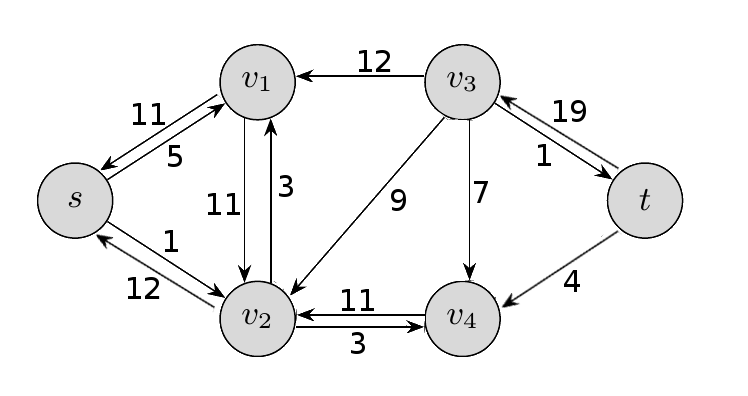
\includegraphics[scale = 0.25]{imagenes/red_residual_5.png}
	\end{center}
	{\small
	¿Hay alg\'un camino de aumento? ¿En cu\'anto se puede aumentar este nuevo flujo? ¿C\'omo se actualiza la nueva red residual?}
\end{frame}

\section{Algoritmos de tipo Ford-Fulkerson}

\begin{frame}{Algunos problemas que pueden ocurrir}
	Si buscamos caminos de aumento en la red residual con DFS, podemos tener el siguiente problema.
	\begin{center}
		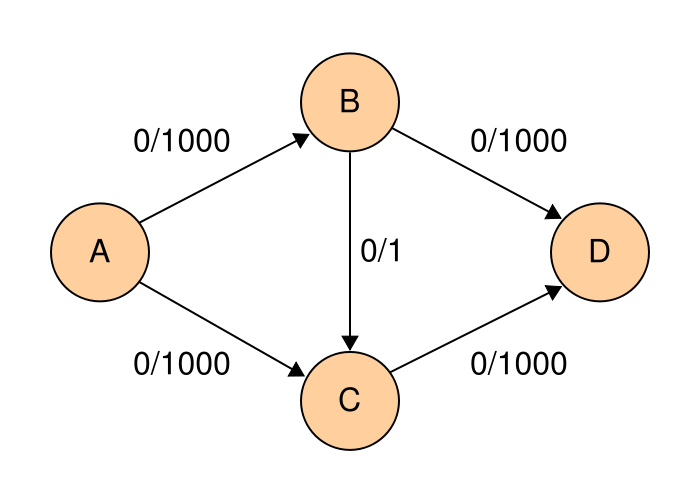
\includegraphics[scale = 0.2]{imagenes/contra_ejemplo.png}
	\end{center}
	\pause
	Si las capacidades son enteras, en cada paso aumentamos el flujo enviado en por lo menos una unidad. Entonces, buscaremos caminos de aumento a lo sumo tantas veces como el valor del m\'aximo flujo en la red.
	\pause
	
	Como asumimos que todos los nodos son alcanzables desde $s$, tenemos por lo menos $|\mathbb{V}|-1$ aristas, y la complejidad total del algoritmo queda acotada por $\mathcal{O} \left ( (|\mathbb{V}|+|\mathbb{E}|)|f^*| \right ) = \mathcal{O}(|\mathbb{E}||f^*|)$
\end{frame}

\begin{frame}{Algoritmo de Edmonds-Karp}
	Si en lugar de buscar con DFS, buscamos caminos de aumento con BFS, la cantidad de veces que buscamos caminos de aumento puede acotarse por una cota que no depende de la respuesta buscada.En el algoritmo de Edmonds-Karp, el camino de aumento elegido es el camino mínimo en cantidad de aristas entre $s$ y $t$ en la red residual. De existir, ese camino se encuentra utilizando BFS.
	
	\pause
	Dado un camino de aumento en la red residual, decimos que una arista es \textit{cr\'itica} si la capacidad m\'inima del camino de aumento se realiza en esa arista. Todo camino de aumento tiene al menos una arista cr\'itica.
	
	\begin{figure}
	    \centering
	    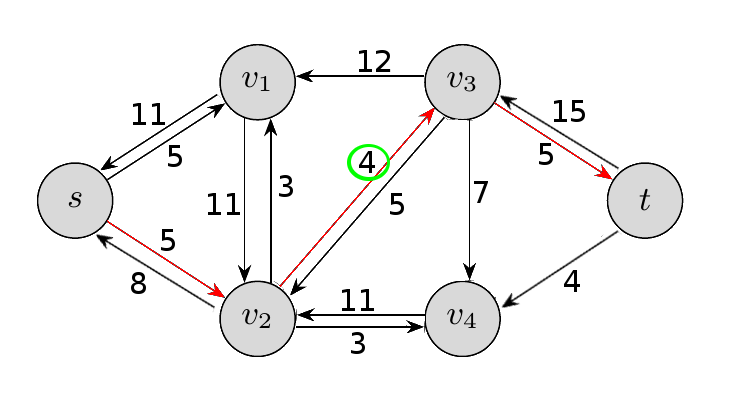
\includegraphics[scale=0.25]{imagenes/red_residual_4.png}
	\end{figure}

\end{frame}

\begin{frame}{Algoritmo de Edmonds-Karp}
	Supongamos que tenemos una arista que conecta dos extremos $u$ y $v$ en nuestra red. Llamamos $u$ al que se encuentra m\'as cerca de $s$ ¿Cu\'antas veces puede ser una arista cr\'itica? 
	\pause 
	
	Notamos $dist^f(u,v)$ como la distancia entre $u$ y $v$ en la red residual correspondiente al flujo $f$.
	
	\pause Si $e = (u,v)$ es cr\'itica, entonces $dist^f(s,v) = dist^f(s,u) + 1$, pues el camino de aumento es m\'inimo en aristas (porque usamos BFS). Adem\'as, una arista cr\'itica no aparece en la pr\'oxima red residual.
	
	Para que la arista $e=(u,v)$ vuelva a aparecer, debe encontrarse primero un camino de aumento que utilice $e' = (v,u)$. Llamaremos $f'$ al flujo en $\mathcal{G}$ donde ocurre esto.
	
	\begin{columns}
	\column{0.5\textwidth}
	\centering
	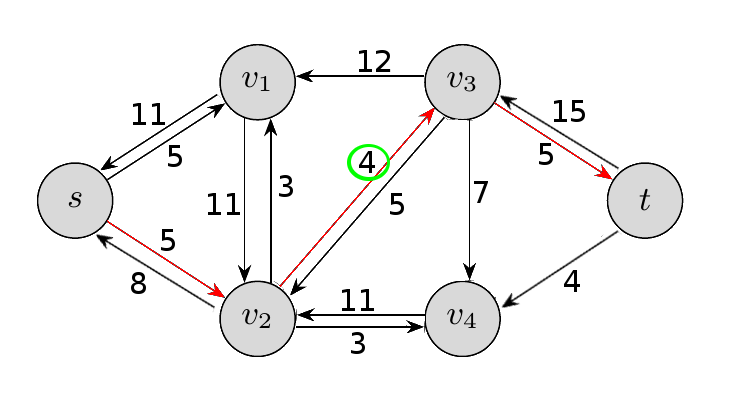
\includegraphics[width=\textwidth]{imagenes/red_residual_4.png}
	\column{0.5\textwidth}
	\centering
	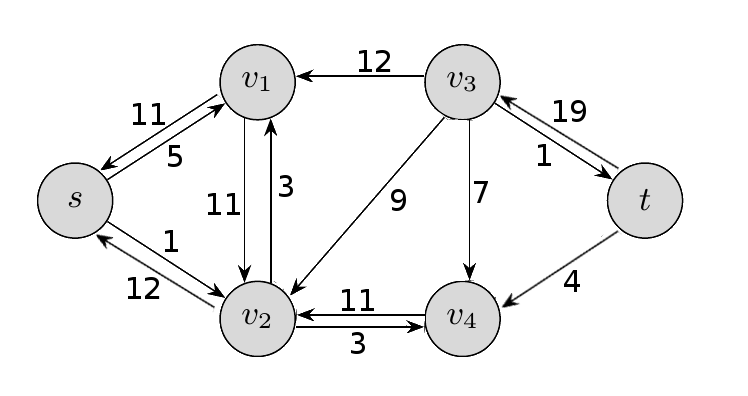
\includegraphics[width=\textwidth]{imagenes/red_residual_5.png}
	\end{columns}

\end{frame}

\begin{frame}{Algoritmo de Edmonds-Karp}
    \small
	Ahora hay que notar dos cosas:
	\begin{itemize}
		\item Como este camino de aumento que usa $e' = (v,u)$ es m\'inimo en aristas, $dist^{f'}(s,u) = dist^{f'}(s,v) + 1$
		\item Los largos de los caminos de aumento son no decrecientes (esto es intuitivo, pero no trivial de demostrar, ver lema 26.7 de ``Introduction to Algorithms''\footnote{Es el lema 26.7 en la tercera edici\'on del libro}), entonces $dist^{f}(s,u) \leq dist^{f'}(s,u)$
	\end{itemize}
	
	\pause
	Juntando estos dos resultados, obtenemos que $dist^{f'}(s,u) = dist^{f'}(s,v) + 1 \geq dist^{f}(s,v) + 1 = dist^{f}(s,u) + 2$ 
	
	Entonces, desde que $e=(u,v)$ es crítica hasta que vuelve a ser crítica, la distancia desde $s$ hasta $u$ en la red residual incrementa en, por lo menos, $2$.\pause Inicialmente, la distancia desde $s$ a $u$ es por lo menos $0$. Como $u\neq t$, los vértices intermedios en el camino mínimo desde $s$ hasta $u$ no pueden contener a $s$, $u$ ni $t$. Luego, a menos que $u$ sea inalcanzable en la red residual, su distancia desde $s$ es a lo sumo $|\mathbb{V}| - 2$. 
	\pause
	
	Por lo tanto, desde la primera vez que $(u,v)$ es crítica, puede volver a ser crítica a lo sumo $(|\mathbb{V}| - 2)/2 = |\mathbb{V}|/2 - 1$ veces. Por ende, puede ser crítica a lo sumo $|\mathbb{V}|/2$ veces.
	\pause
	Buscar un camino de aumento tiene una complejidad de $\mathcal{O}(|\mathbb{E}|)$. Si se realiza a lo sumo $\frac{|\mathbb{E}||\mathbb{V}|}{2}$ veces, la complejidad total del algoritmo resulta $\mathcal{O}(|\mathbb{E}|^2|\mathbb{V}|)$ 
	
	\medskip
\end{frame}

\begin{frame}{Algoritmo de Edmonds-Karp}
	
	A lo largo del algoritmo utilizaremos:
	\begin{itemize}
		\item $\texttt{f[u][v]}$: Como el flujo actual que va de $u$ a $v$
		\item $\texttt{c[u][v]}$: Como la capacidad de la arista de $u$ a $v$ en $\mathcal{R}_{\mathcal{G}}$. Se inicializa con las capacidades originales en $\mathcal{G}$
	\end{itemize}
	Edmonds-Karp$(\mathcal{G},s,t)$ ($\mathcal{G}$ alguna representaci\'on del grafo)
	\begin{enumerate}
		\item $\forall e = (u,v) \in \mathbb{E}:$
		\begin{enumerate}
			\item $\texttt{f[u][v]} \leftarrow 0$
		\end{enumerate}
		\item $\mathcal{P} \leftarrow \text{BFS}^{\bigstar}(\mathcal{R}_{\mathcal{G}},s,t)$ \textcolor{Mahogany}{\scriptsize $\Leftarrow  \boxed{\text{Camino de aumento de } s \text{ a } t\hspace{2pt} (\text{o }\varnothing\text{ si no existe})}$}
		\item Mientras $\mathcal{P} \neq \varnothing$:
		\begin{enumerate}
			\item $\texttt{valor\_critico} \leftarrow \min \{ \texttt{c[u][v]} : e = (u,v) \in \mathcal{P} \}$
			\item $\forall e =(u,v) \in \mathcal{P}$:
			\begin{enumerate}
				\item $\texttt{c[u][v]} \leftarrow \texttt{c[u][v]-valor\_critico}$
				\item $\texttt{f[u][v]} \leftarrow \texttt{f[u][v]+valor\_critico}$
				\item $\texttt{c[v][u]} \leftarrow \texttt{c[v][u]+valor\_critico}$ 
			\end{enumerate}
			\item $\mathcal{P} \leftarrow \text{BFS}^{\bigstar}(\mathcal{R}_{\mathcal{G}},s,t)$
		\end{enumerate}
	\end{enumerate}
\end{frame}

\begin{frame}{Flujo m\'aximo de m\'inimo costo}
    \small
	Ya vimos c\'omo obtener el m\'aximo flujo en una red. Ahora supongamos que en cada arista, adem\'as de tener una cierta capacidad tengo un costo \textbf{por unidad de flujo} enviado por dicha arista.
	
	El problema que tendremos ahora ser\'a encontrar de todos los flujos de m\'aximo valor, alguno que minimice el costo asociado a dicho flujo. En otras palabras, si $r(u,v)$ es el costo por unidad de flujo, ahora buscamos entre todos los flujos de valor m\'aximo, a alguno que minimice:
	$$ \sum\limits_{e = (u,v) \in \mathbb{E}} f(u,v)\cdot r(u,v)$$
	
	¿C\'omo podemos resolver esto?
	
	\pause
	Hacemos lo mismo que antes, pero en vez de buscar caminos de aumento con BFS, ahora lo haremos con Bellman-Ford. Notemos que al actualizar la red residual hay que tener cuidado, pues al dejar de enviar flujo entre dos v\'ertices, el 'costo' ser\'a el inverso del de enviar el flujo entre dichos v\'ertices.
	
	\begin{columns}
	\column{0.5\textwidth}
	\only<2>{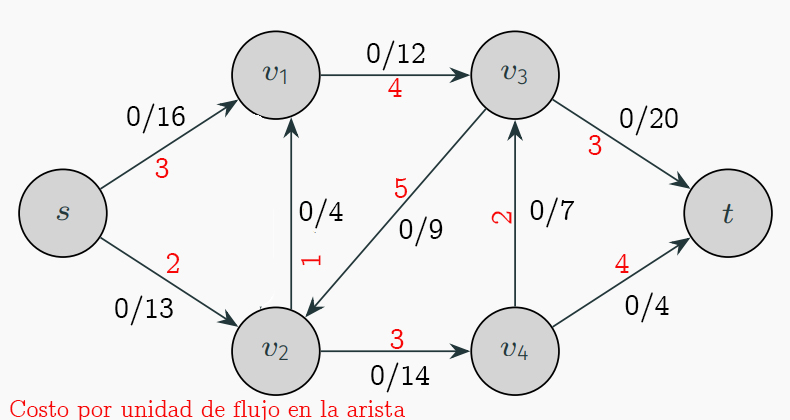
\includegraphics[width=\textwidth]{imagenes/red0.jpg}}
	\only<3>{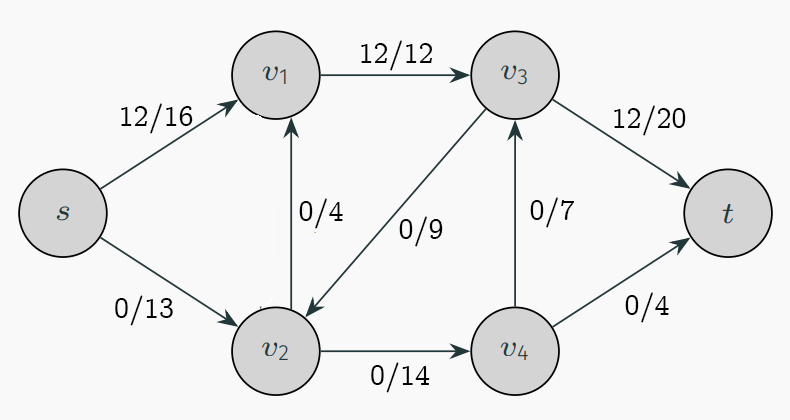
\includegraphics[width=\textwidth]{imagenes/red1.jpg}}
	\column{0.5\textwidth}
	\only<2>{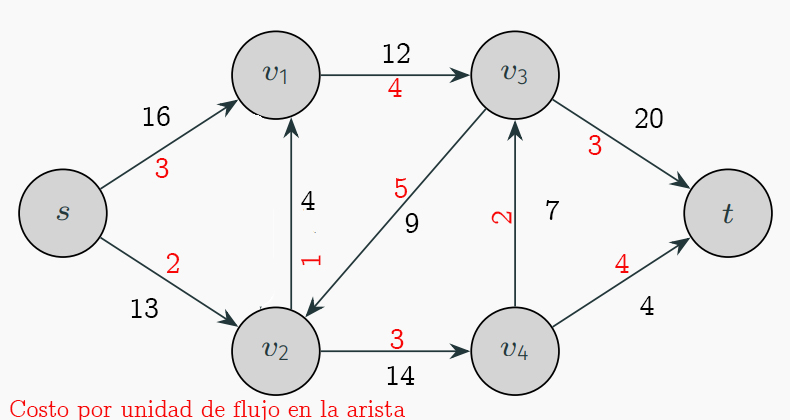
\includegraphics[width=\textwidth]{imagenes/res0.jpg}}
	\only<3>{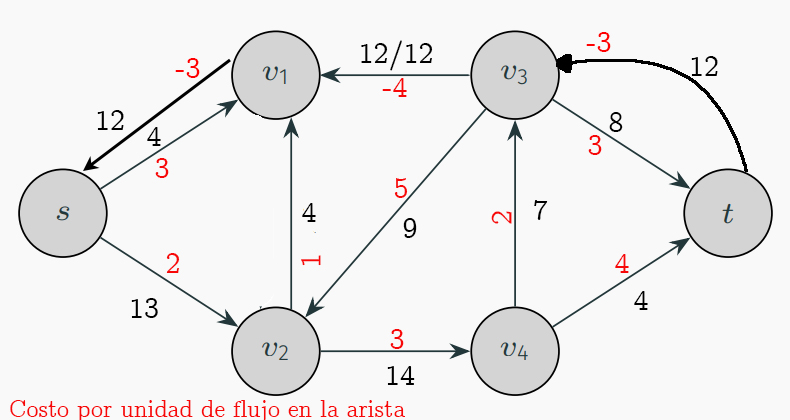
\includegraphics[width=\textwidth]{imagenes/res1.jpg}}
	\end{columns}
\end{frame}

\begin{frame}{Matching de costo m\'inimo}
	Imaginemos que tenemos $N$ posibles trabajadores y $M$ tareas a ser completadas en simult\'aneo, con $N \geq M$. El $i$-\'esimo trabajador pide una remuneraci\'on de $r(i,j)$ por realizar el $j$-\'esimo trabajo.
	
	¿Qu\'e trabajadores debemos seleccionar para realizar cada trabajo?¿C\'omo lo modelamos en t\'erminos de alguna red de flujo apropiada?
	
	\pause
	
	Si $N = M$ existen algoritmos m\'as eficientes para resolver este problema, como por ejemplo el $\textit{algoritmo h\'ungaro}$. 
\end{frame}

% \begin{frame}{Algoritmo de Dinitz (conocido tambi\'en como Dinic)}
% 	La idea detr\'as de este algoritmo es aprovechar toda la informaci\'on que tenemos a la hora de correr el algoritmo de Edmonds-Karp. La cota en la cantidad de veces que se buscan caminos de aumento radica en que se buscan caminos de que minimicen la cantidad de aristas (por eso usa BFS). 
	
% 	Ahora, una vez que hacemos un BFS tenemos la distancia de cada nodo al nodo fuente $s$, entonces ¿por qu\'e quedarnos con un solo camino?
	
% 	\pause
% 	Para cada nodo calculamos su distancia al nodo $s$. La idea central ahora ser\'a solo movernos por aristas que aumenten en $1$ la distancia respecto del nodo actual. Si ahora recorremos en forma ordenada con $DFS$, una vez que llegamos a $t$, habremos llegado necesariamente por un camino que minimiza la cantidad de aristas usadas. Algunas aristas de este camino son cr\'iticas, ¿desde d\'onde podemos seguir el recorrido de DFS?
	
% 	\pause
	
% 	Podemos seguir buscando caminos de aumento desde el extremo m\'as cercano a $s$ de la arista cr\'itica m\'as cercana a $s$ al retrotraer en el mismo DFS. 
	 
% \end{frame}

% \begin{frame}{Algoritmo de Dinitz (conocido tambi\'en como Dinic)}
% 	Al hacer esto, en la pr\'oxima iteraci\'on la distancia de $s$ a $t$ aument\'o en uno (no pueden haber quedado caminos que minimizaban la cantidad de aristas), por lo tanto, ahora podemos acotar por $\mathbb{|V|}-1$ la cantidad de veces que buscamos caminos de aumento en vez de $\frac{|\mathbb{E}||\mathbb{V}|}{2}$, por lo tanto la complejidad total del algoritmo nos queda \dots \pause $\mathcal{O}(|\mathbb{V}|^2|E|)$
% 	\pause La observaci\'on es que al retrotraer en el DFS, si bien algunas aristas se fueron, \textbf{podemos volver a visitar los mismos nodos} de antes. Lo que s\'i vale es que desde cada nodo, a lo sumo se visita cada arista una vez.
% \end{frame}

\end{document}

